\chapter{Ergebnisse}
\label{chap:ergebnisse}

Nachdem in \autoref{chap:umsetzung} bereits die technische Erklärung der einzelnen Bestandteile erfolgte, werden nun die für den Anwender wichtigen Ergebnisse innerhalb des \textit{Jenkins} \ac{ui} dargestellt.

\section{\acl{ui} des Plugins} 

Das \textit{Plugin} bietet, wie in \autoref{chap:actions} eingeführt, zwei \textit{Actions} mit einer \ac{ui}-Komponente. Eine Übersicht über alle \textit{Pull Requests} auf erster \textit{Job}-Ebene und das eigentliche \textit{Dashboard} auf der \textit{Run}-Ebene.

\subsection{\textit{Job}-Ansicht}
\label{chap:job-result}

Für jeden \textit{Pull Request} werden der Name des \textit{Pull Requests}, der Name des Mitwirkenden und sowohl der Quell- als auch der Ziel-\textit{Branch} aufgelistet, wie \autoref{fig:overview} zeigt. 

\begin{figure}[h!]
\centering
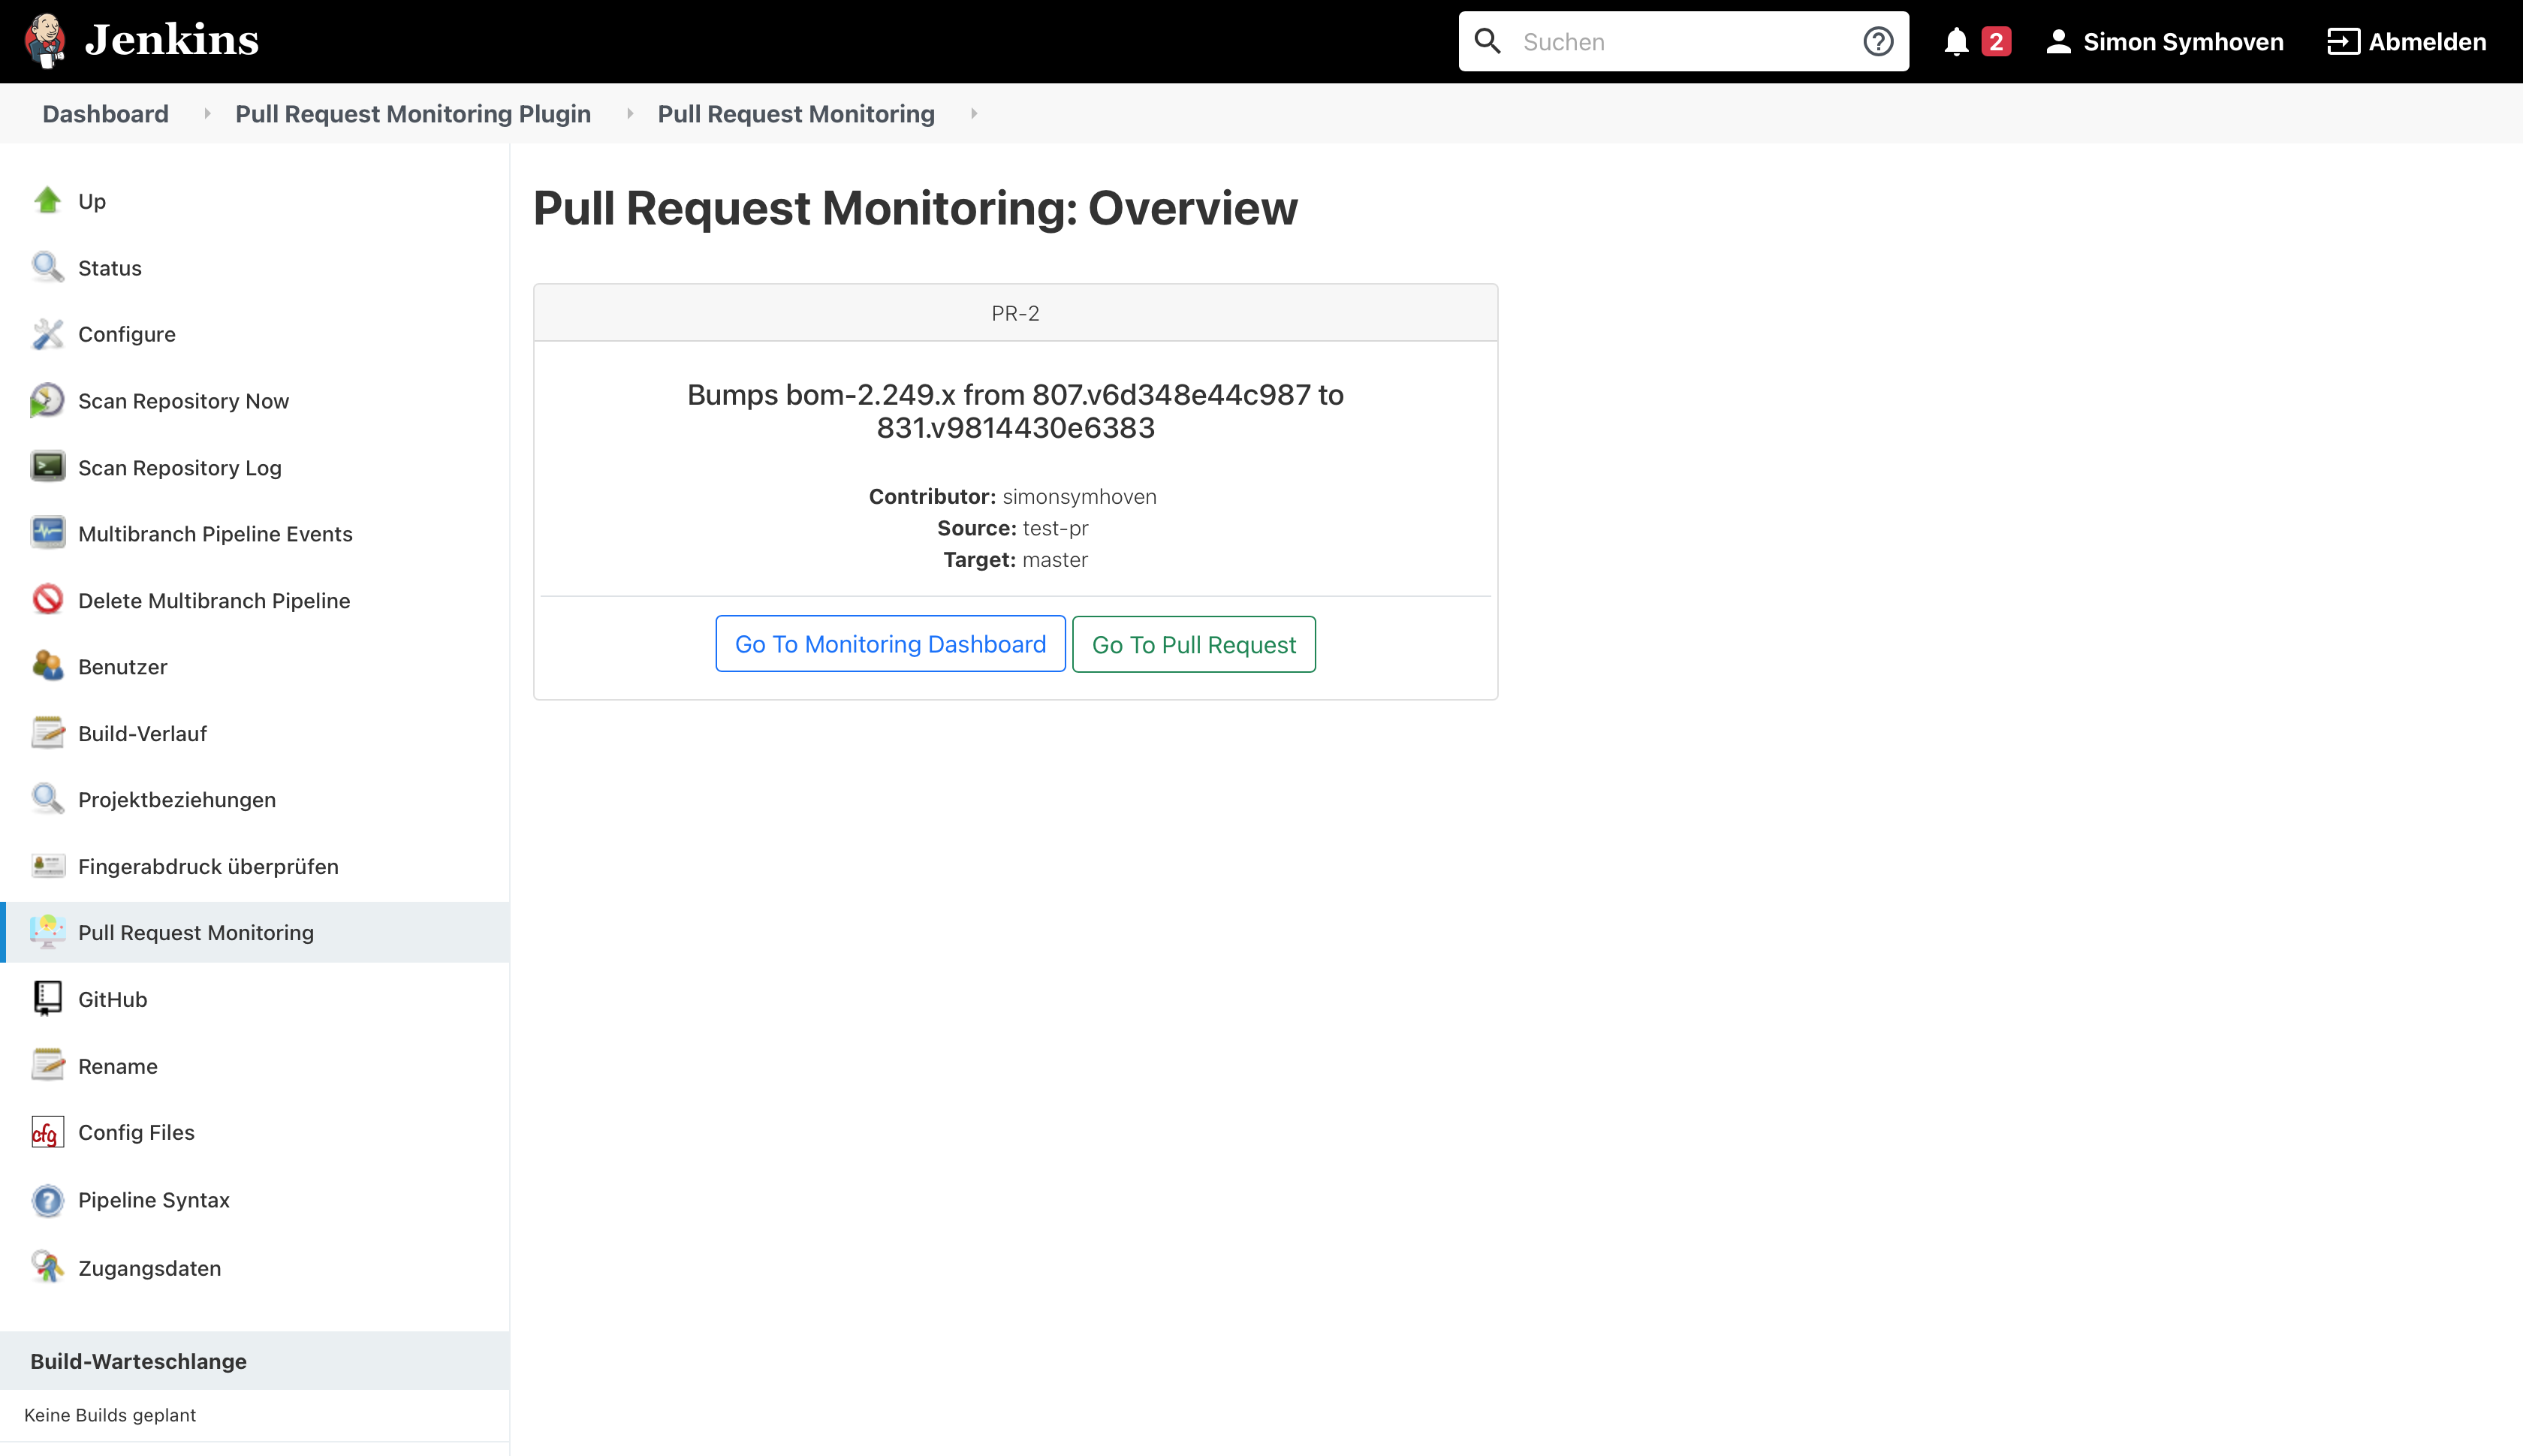
\includegraphics[width=\textwidth]{source/images/overview}
\caption[\textit{MonitoringMultibranchProjectAction} auf erster \textit{Job}-Ebene: Übersicht aller \textit{Pull Requests}.]{\textit{MonitoringMultibranchProjectAction} auf erster \textit{Job}-Ebene: Übersicht aller \textit{Pull Requests}, Quelle: Eigene Aufnahme.}
\label{fig:overview}
\end{figure}

Von hier aus kann entweder zu der \ac{ui}-Komponente des letzten zugehörigen \textit{Runs}, also der \textit{Run}-Ansicht aus \autoref{chap:build-result} mit dem \textit{Dashboard} navigiert werden oder der \textit{Pull Request} im \ac{scm}-System, z.\,B. \textit{GitHub} geöffnet werden.


\subsection{\textit{Run}-Ansicht}
\label{chap:build-result}

Das \textit{Dashboard} besteht aus verschiedenen Einheiten. Einem Titel, den Metadaten eines \textit{Pull Requests}, dem \textit{Muuri} Layout mit den \textit{Portlets} und zwei Schaltflächen, um neue \textit{Portlets} hinzuzufügen und die Einstellungen zu öffnen. 

\begin{figure}[h!]
\centering
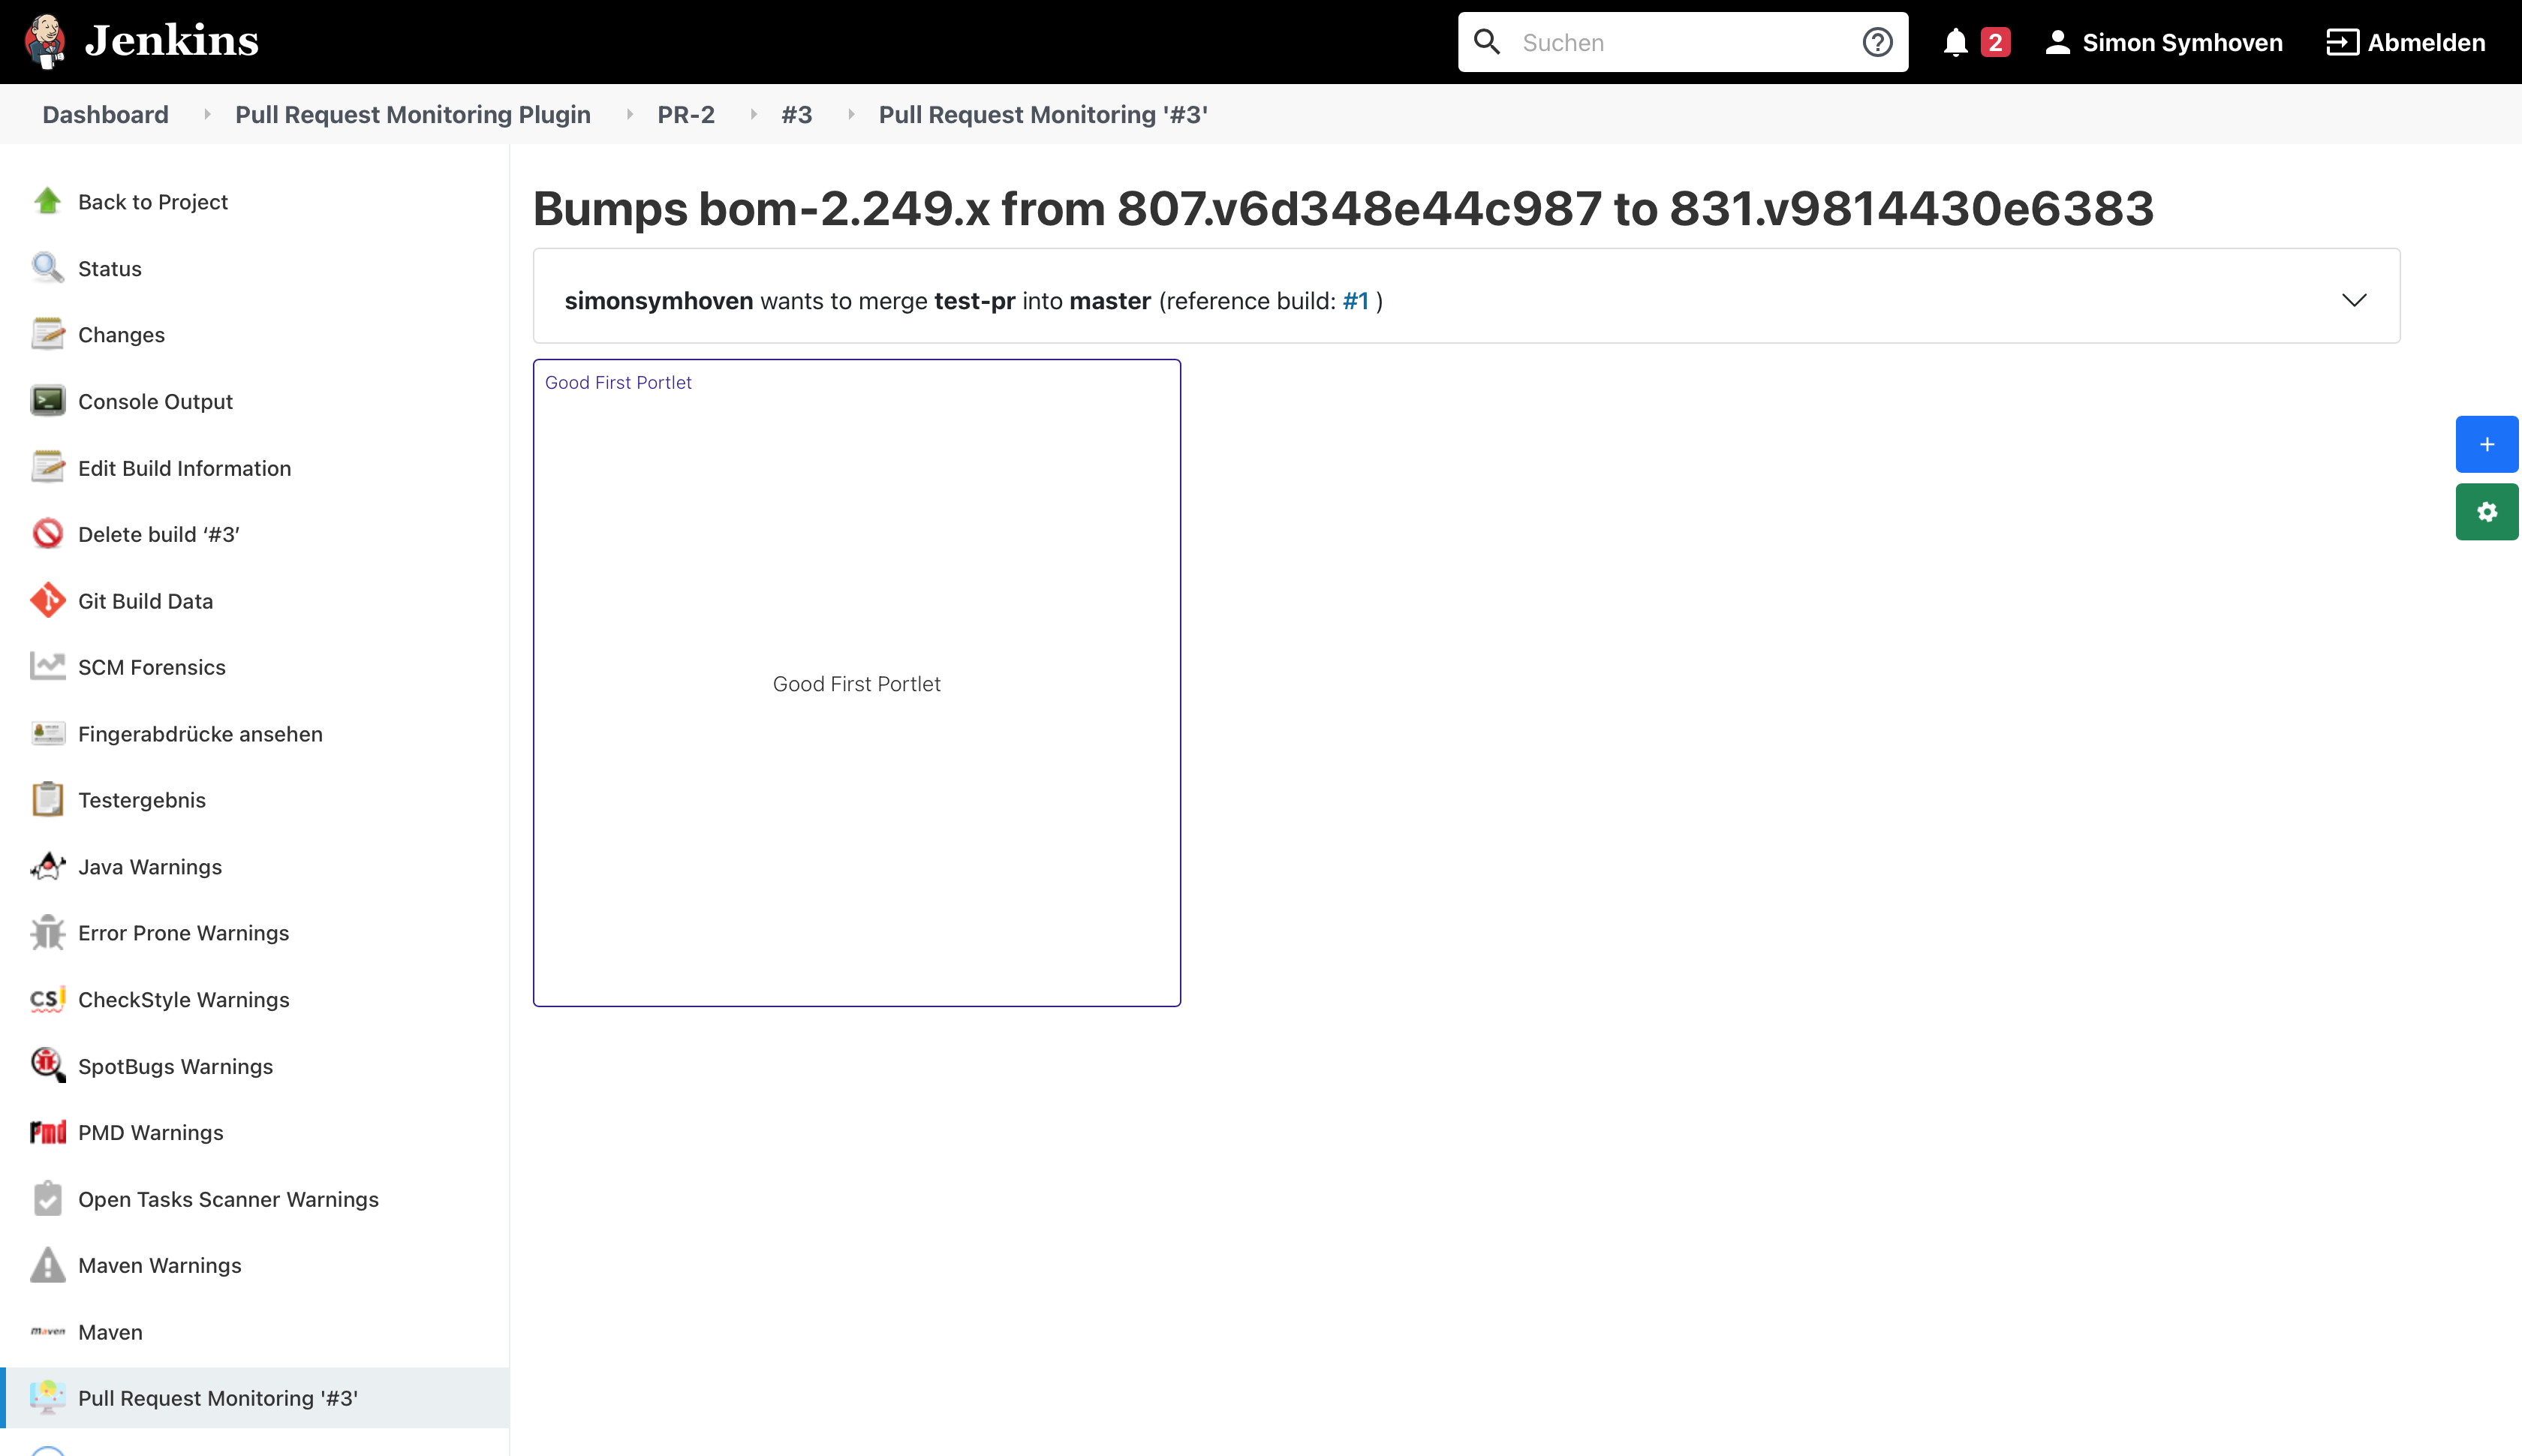
\includegraphics[width=\textwidth]{source/images/build}
\caption[\textit{MonitoringDefaultAction} auf \textit{Run}-Ebene: Das \textit{Dashboard}.]{\textit{MonitoringDefaultAction} auf \textit{Build}-Ebene: Das \textit{Dashboard}, Quelle: Eigene Aufnahme.}
\label{fig:build}
\end{figure}

Die \textit{Portlets} innerhalb des \textit{Muuri} Layouts aus \autoref{fig:build} können per \textit{Drag \& Drop} beliebig verschoben werden oder mit einem Klick auf die rechte obere Ecke des jeweiligen \textit{Portlets} gelöscht werden.

\subsubsection{Metadaten eines \textit{Pull-Requests}}

Analog zu der Übersicht der \textit{Pull Requests} aus \autoref{chap:job-result} werden auf \textit{Run}-Ebene alle Metadaten des \textit{Pull Requests} angezeigt. Außerdem wird der Referenz-\textit{Run} des zugehörigen Ziel-\textit{Branches} angegeben. Zusätzlich wird, falls vorhanden, die Beschreibung aus dem \ac{scm}-System ausgegeben, wie \autoref{fig:metadata} zeigt:

\begin{figure}[h!]
\centering
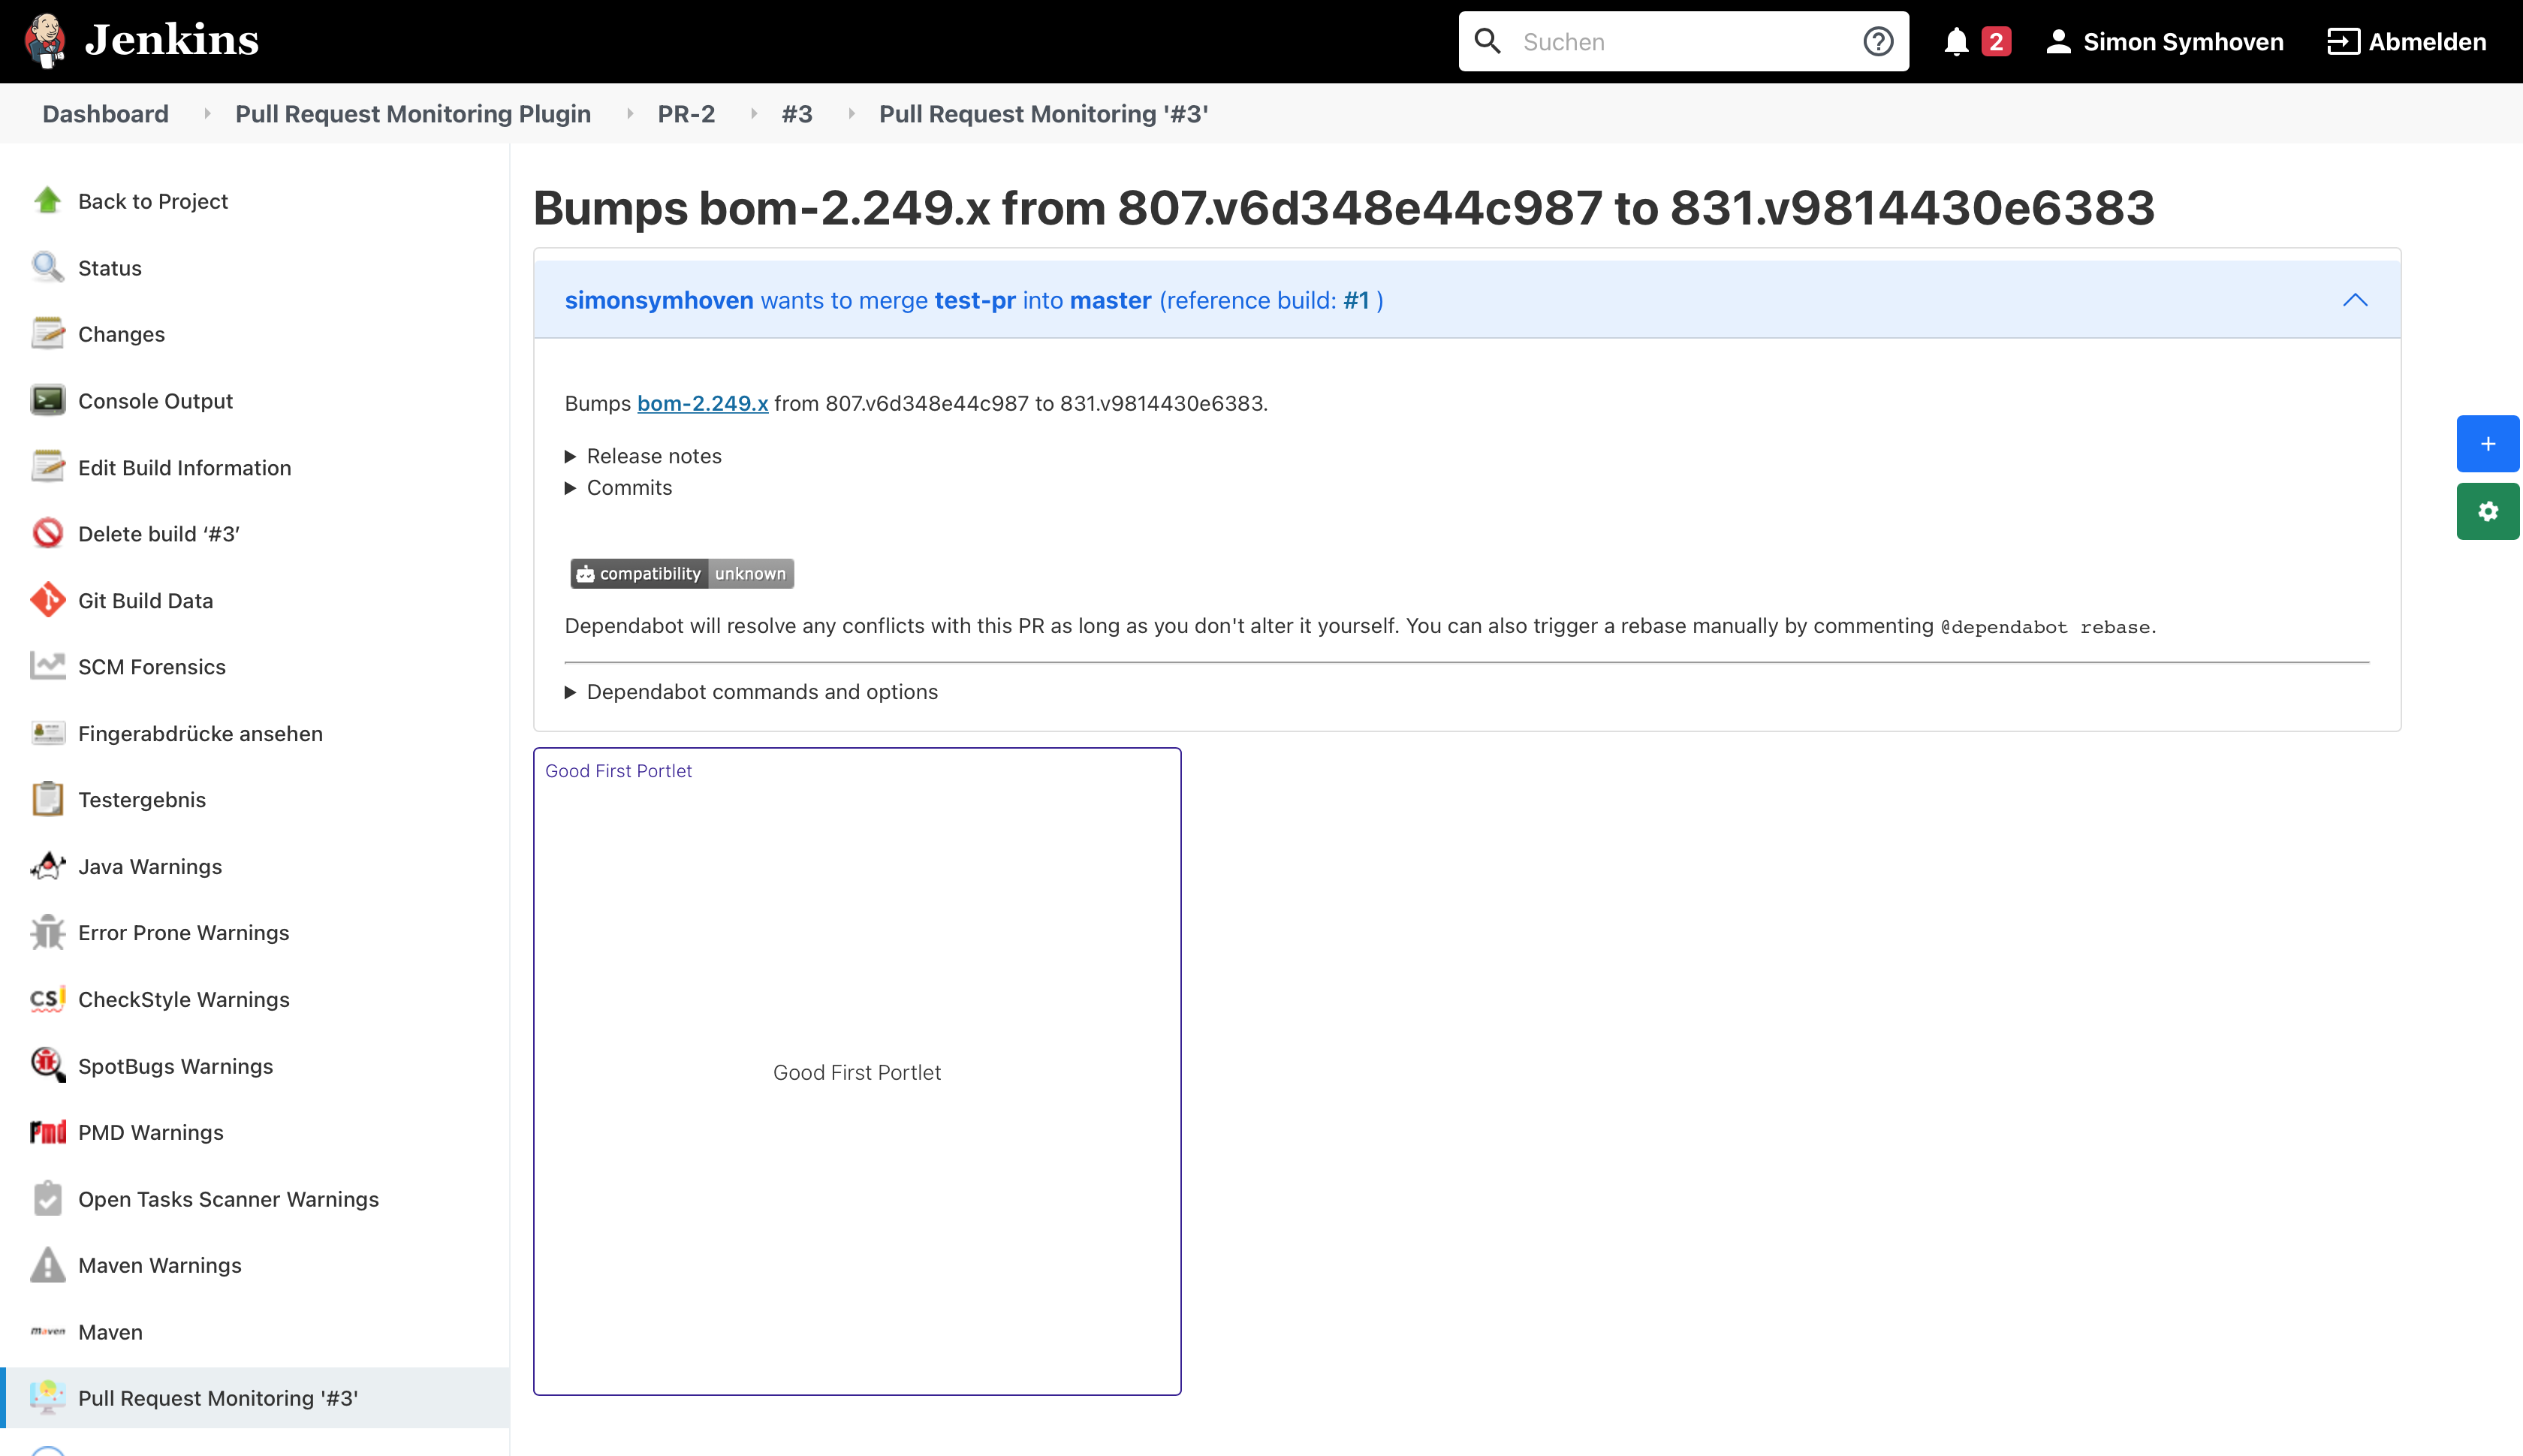
\includegraphics[width=\textwidth]{source/images/metadata}
\caption[Metadaten eines \textit{Pull Requests}.]{Metadaten eines \textit{Pull Requests}, Quelle: Eigene Aufnahme.}
\label{fig:metadata}
\end{figure}

\subsubsection{\textit{Portlets} hinzufügen}
\label{chap:add}

Um ein neues \textit{Portlet} hinzuzufügen, muss zunächst aus der Liste der verfügbaren \textit{Portlets} eines ausgewählt werden, wie \autoref{fig:add1} zeigt. Ist dieses bereits im Layout enthalten, so wird das entsprechende \textit{Portlet} ausgegraut. Falls gewünscht, kann die vordefinierte Breite und Höhe des ausgewählten \textit{Portlets} modifiziert und überschrieben werden. Auch die Farbe kann verändert werden. \autoref{fig:add2} zeigt die Einstellungen für das selektierte \textit{Java} \textit{Portlet} aus dem \textit{Warnings Next Generation Plugin}.

\begin{figure}[h!]
\begin{minipage}[t]{0.49\textwidth}
\centering
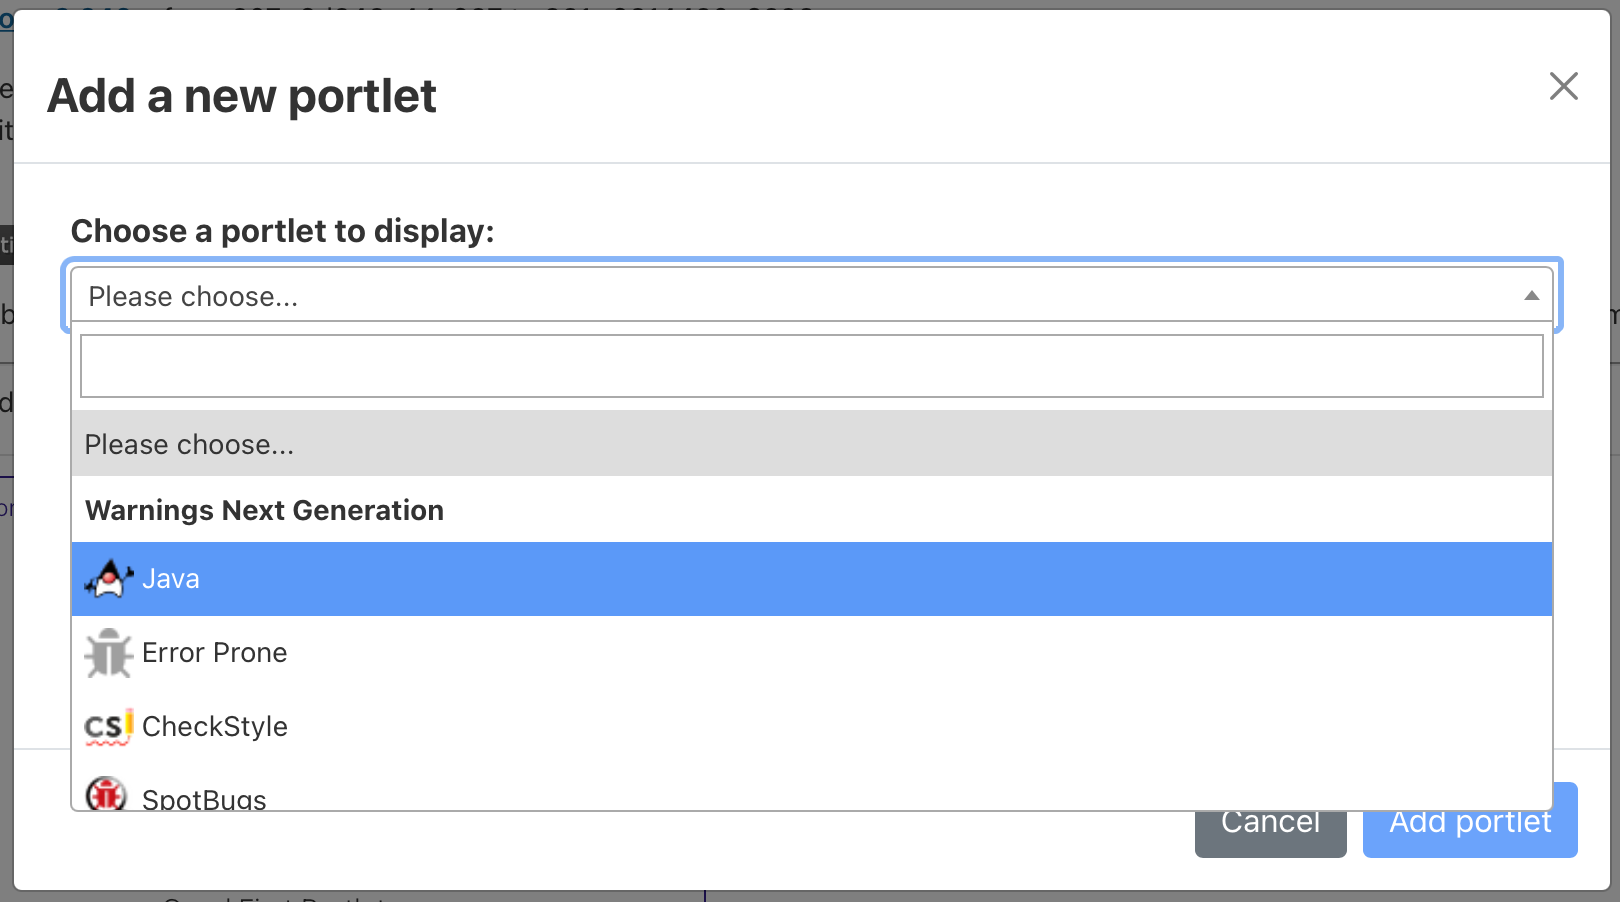
\includegraphics[width=\textwidth]{source/images/add1}
\caption[Ein neues \textit{Portlet} hinzufügen. Auswahl des \textit{Portlets}.]{Ein neues \textit{Portlet} hinzufügen. Auswahl des \textit{Portlets}, Quelle: Eigene Aufnahme.}
\label{fig:add1}
\end{minipage}
\hspace{0.1cm}
\begin{minipage}[t]{0.49\textwidth}
\centering
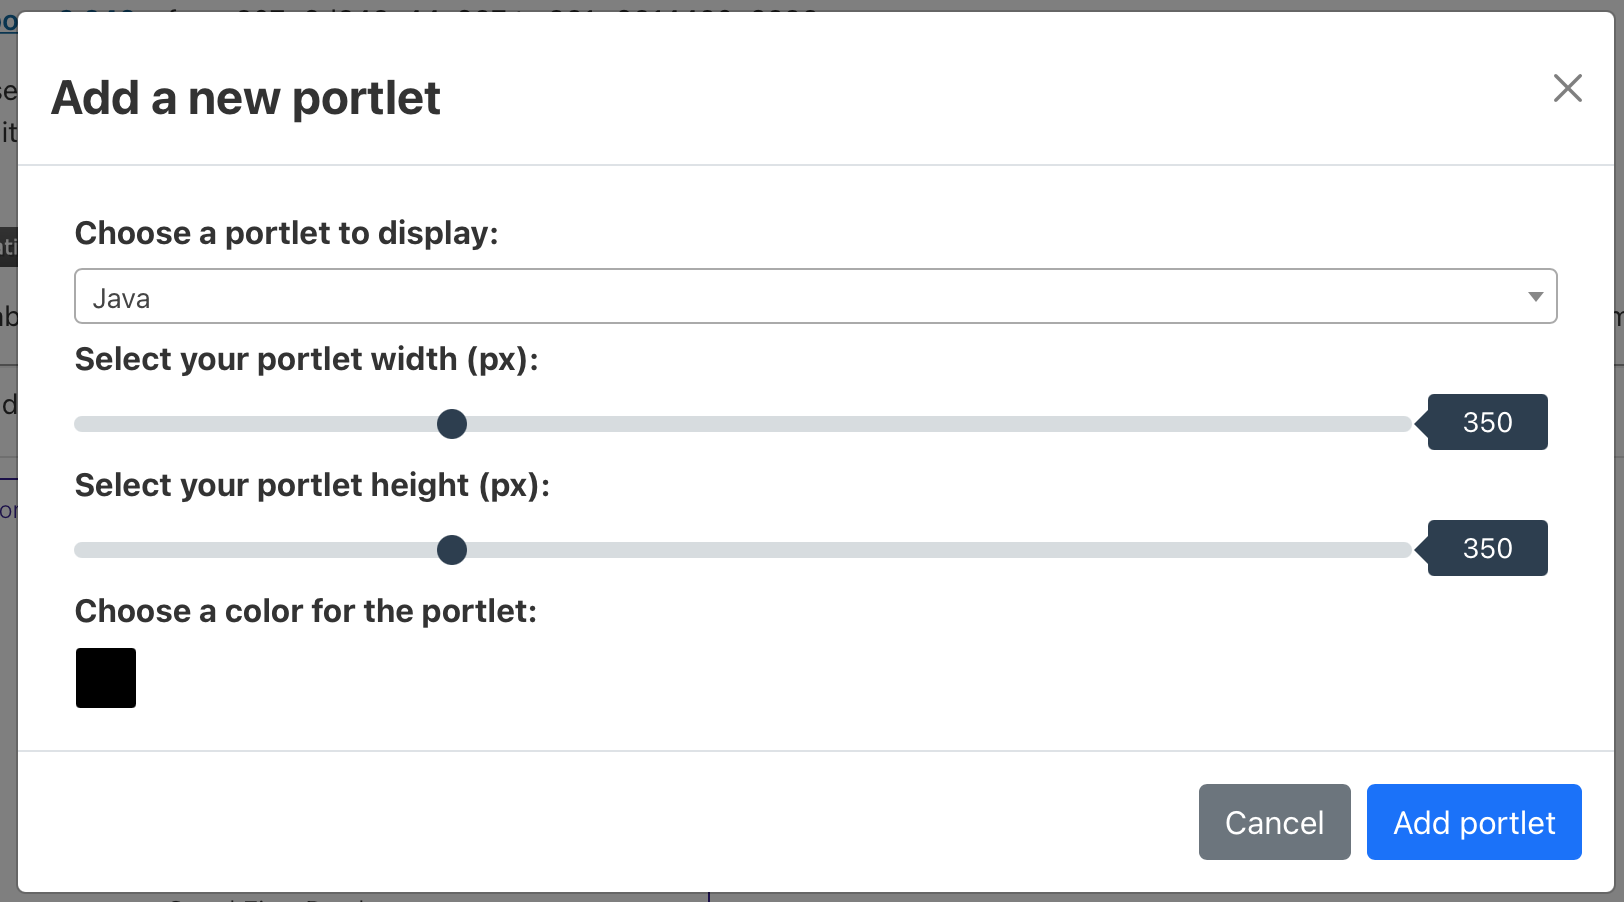
\includegraphics[width=\textwidth]{source/images/add2}
\caption[Ein neues \textit{Portlet} hinzufügen. Auswahl der Größe und Farbe.]{Ein neues \textit{Portlet} hinzufügen. Auswahl der Größe und Farbe, Quelle: Eigene Aufnahme.}
\label{fig:add2}
\end{minipage}
\end{figure}


\subsubsection{Einstellungen}
\label{chap:settings}

Die Einstellungen aus \autoref{fig:settings} bieten dem Nutzer die Möglichkeit, bestimmte Informationen über das Dashboard einzusehen. Es wird ermittelt, ob es Änderungen an der Konfiguration in der \textit{Pipeline} seit dem letzten \textit{Run} gibt und die Quelle der Konfiguration angezeigt. Diese kann entweder \textit{Default} oder \textit{User-Specific} sein. Außerdem wird berechnet, ob die aktuelle Konfiguration mit der \textit{default}-Konfiguration übereinstimmt. Der Anwender hat die Möglichkeit, die aktuelle Konfiguration zu jeder Zeit auf die \textit{default}-Konfiguration zurückzusetzen. Die beiden Konfiguration werden außerdem als \textit{JSON-Tree} mit ihren Attributen abgebildet. 

\begin{figure}[h!]
\centering
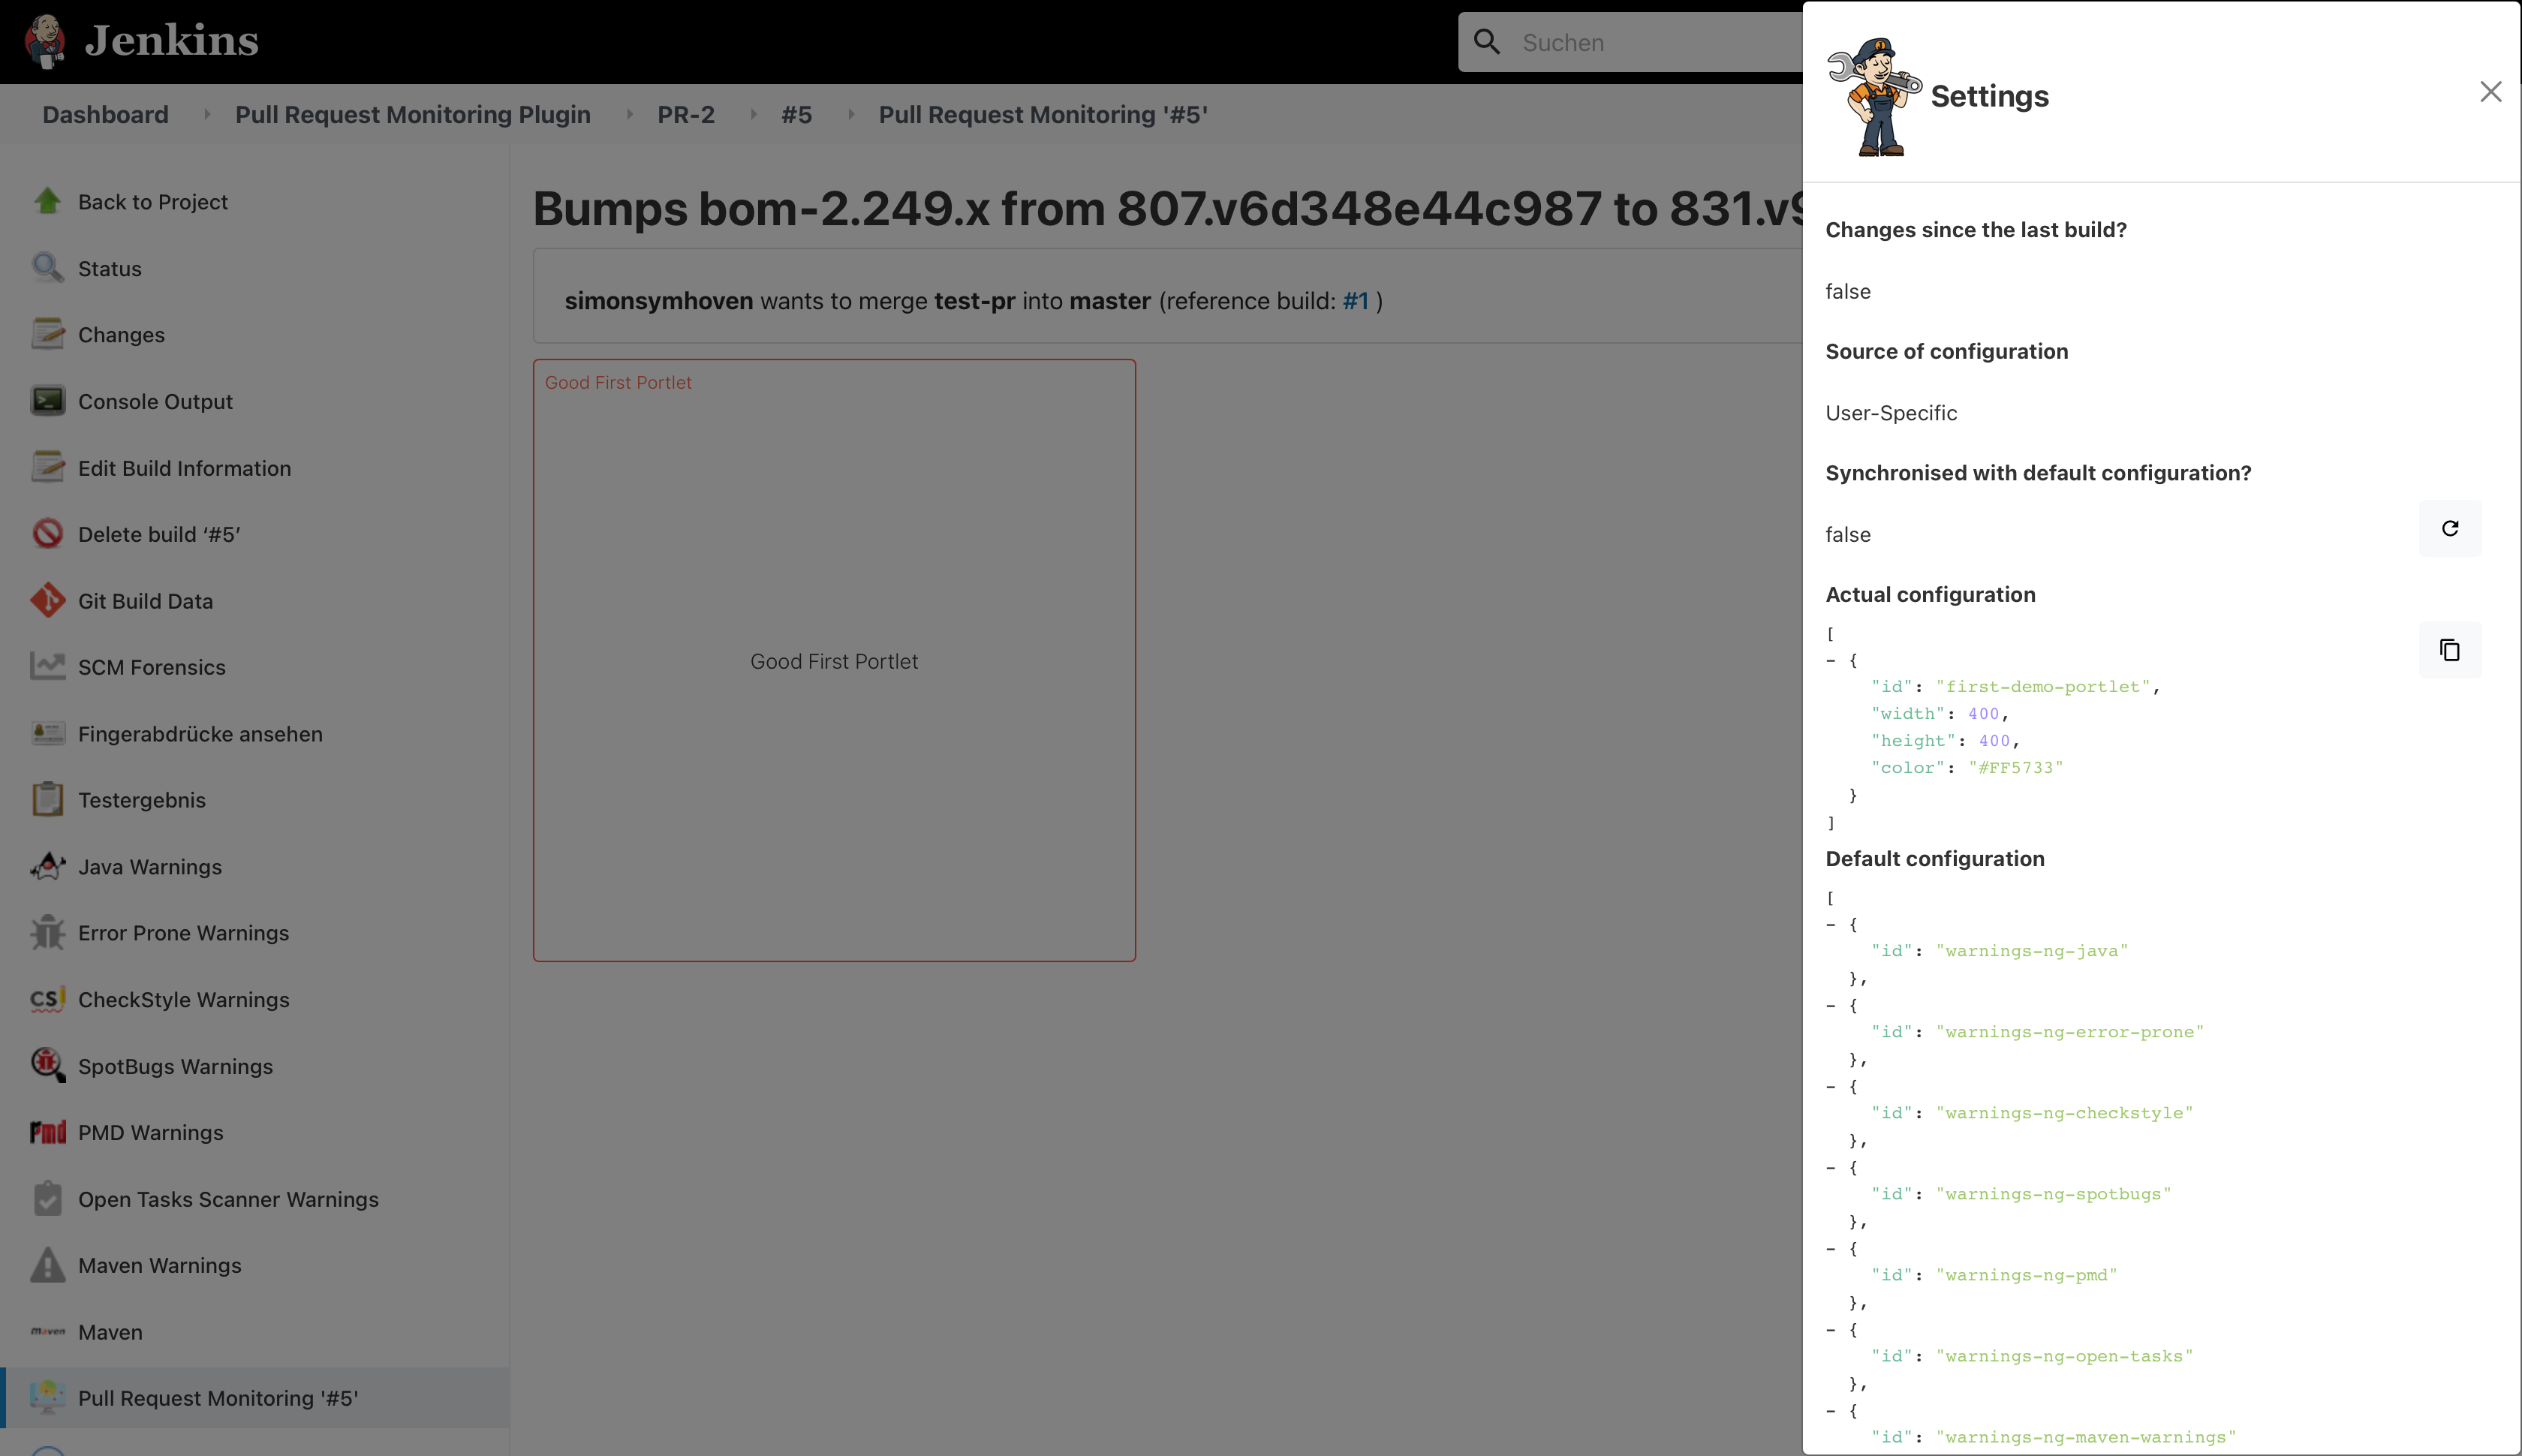
\includegraphics[width=\textwidth]{source/images/settings}
\caption[Ansicht: Einstellungen.]{Ansicht: Einstellungen, Quelle: Eigene Aufnahme.}
\label{fig:settings}
\end{figure}


\section{Verfügbare \textit{Portlets}}

Neben dem \textit{Plugin} selbst wurde während der Entwicklung der vorliegenden Arbeit das entwickelte \ac{api} verwendet, um zwei dieser \textit{Portlets} in anderen \textit{Jenkins} \textit{Plugins} zu entwickeln. So konnte das \ac{api} auf Tauglichkeit geprüft werden und erleichtert das Entwickeln weiterer \textit{Portlets} für andere \textit{Plugin} Betreiber.

\subsection{\textit{Warnings Next Generation Plugin}}
\label{chap:warnings-ng}

\flqq{Das \textit{Warnings Next Generation Plugin} sammelt Compiler-Warnungen oder Probleme, die von statischen Analysewerkzeugen gemeldet werden, und visualisiert die Ergebnisse. Es hat eingebaute Unterstützung für mehr als hundert Berichtsformate.\frqq{}, schreibt \citet{warnings-ng-plugin} über sein \textit{Plugin}. Das \textit{Warnings Next Generation Plugin} liefert für jedes dieser Analysewerkzeuge mithilfe der \textit{MonitorPortletFactory} ein \textit{Portlet} aus. Die grafische Darstellung der Ergebnisse unterscheidet sich von \textit{Portlet} zu \textit{Portlet} nicht - lediglich die zugrundeliegenden Daten ändern sich. Somit wird eine Klasse \textit{MonitorPortlet} verwendet und für jedes Analysewerkzeug eine Instanz dieser Klasse mit den spezifischen Ergebnissen ausgeliefert. Dabei werden drei Fälle unterschieden:

\begin{enumerate}
	\item	Es liegen keine Warnungen vor (\autoref{fig:warning1}).
	\item Es gibt keine neuen Warnungen, aber ausstehende und eventuell gelöste Warnungen (\autoref{fig:warning2}).
	\item Es gibt neue Warnungen. Dazu eventuell ausstehende und gelöste Warnungen (\autoref{fig:warning3}).
\end{enumerate}

\begin{figure}[H]
\begin{minipage}[t]{0.45\textwidth}
\centering
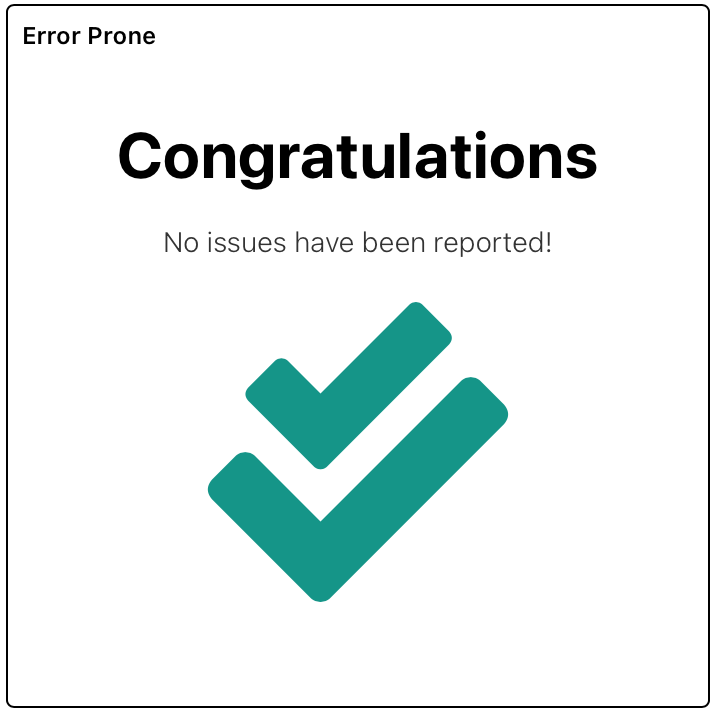
\includegraphics[width=\textwidth]{source/images/warning1}
\caption[\textit{Portlet} des \textit{Warnings Next Generation Plugins} ohne Warnungen.]{\textit{Portlet} des \textit{Warnings Next Generation Plugins} ohne Warnungen, Quelle: Eigene Aufnahme.}
\label{fig:warning1}
\end{minipage}
\hspace{0.5cm}
\begin{minipage}[t]{0.45\textwidth}
\centering
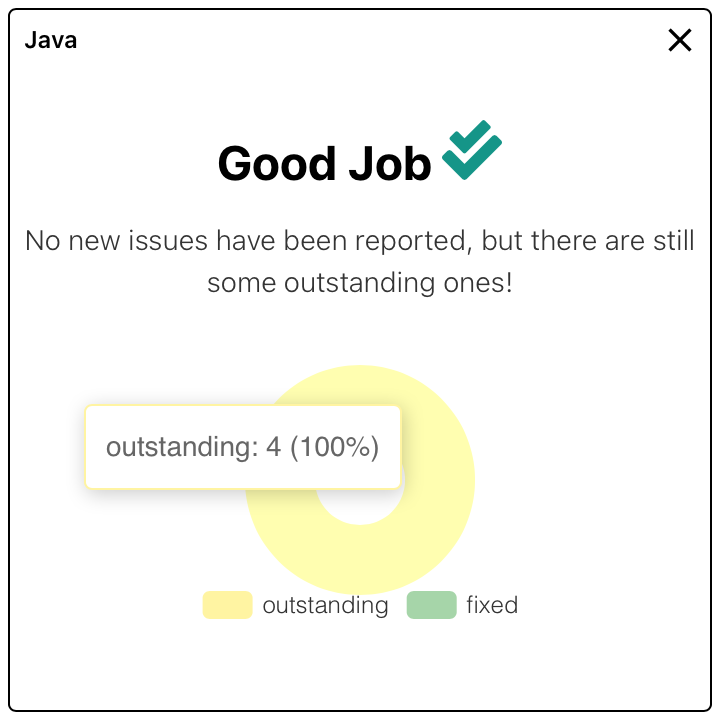
\includegraphics[width=\textwidth]{source/images/warning2}
\caption[\textit{Portlet} des \textit{Warnings Next Generation Plugins} ohne neue Warnungen .]{\textit{Portlet} des \textit{Warnings Next Generation Plugins} ohne neue Warnungen, Quelle: Eigene Aufnahme.}
\label{fig:warning2}
\end{minipage}

\begin{minipage}[t]{0.45\textwidth}
\centering
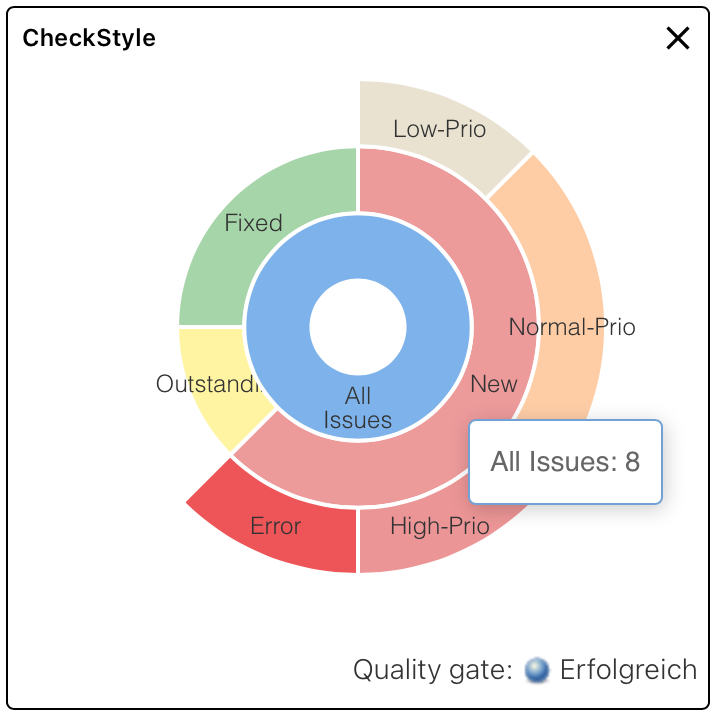
\includegraphics[width=\textwidth]{source/images/warning3}
\caption[\textit{Portlet} des \textit{Warnings Next Generation Plugins} mit Warnungen.]{\textit{Portlet} des \textit{Warnings Next Generation Plugins} mit Warnungen, Quelle: Eigene Aufnahme.}
\label{fig:warning3}
\end{minipage}
\end{figure}

\subsection{\textit{Code Coverage API Plugin}}
\label{chap:code-coverage-api}

Das \textit{Code Coverage API Plugin} dient als \ac{api} zur Integration und Veröffentlichung mehrerer \textit{Coverage Reports} \citep{code-coverage-api-plugin}. Das \textit{Portlet} visualisiert die \textit{Conditional}- und \textit{Line}-\textit{Coverage} bezogen auf den aktuellen \textit{Run} und erzeugt aus den Metriken ein Balkendiagramm. Zusätzlich wird die Differenz zu dem Referenz-\textit{Run} kalkuliert und als Delta hinter der jeweiligen \textit{Coverage} ausgegeben. Die absolute \textit{Conditional}- und \textit{Line}-\textit{Coverage} aus dem \textit{Run} beträgt 78,57 \% bzw. 81,82 \%. Die Delta-\textit{Coverage} bezogen auf den Referenz-\textit{Run} des Ziel-\textit{Branches} hat sich nicht verändert. Die \textit{Code Coverage} (\textit{Conditional} und \textit{Line}) ist folglich in Quell- und Ziel-\textit{Branch} dieselbe und wird durch den \textit{Pull Request} nicht vermindert oder verbessert.

\begin{figure}[H]
\centering
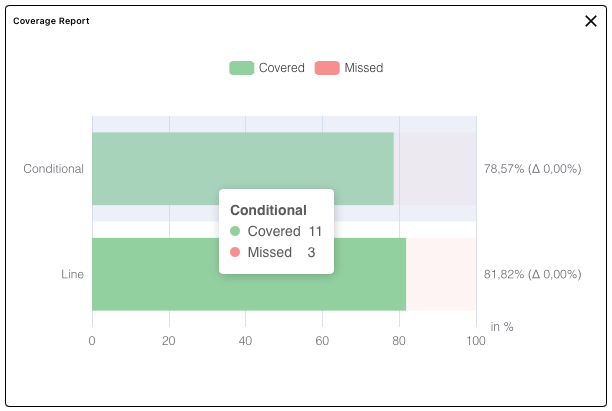
\includegraphics[width=\textwidth]{source/images/coverage}
\caption[\textit{Portlet} des \textit{Code Coverage API Plugins}.]{\textit{Portlet} des \textit{Code Coverage API Plugins}, Quelle: Eigene Aufnahme.}
\label{fig:coverage}
\end{figure}
